\pagestyle{fancy}
\renewcommand{\theUnit}{6}
\ifthenelse{\isundefined{\UnitPageNumbers}}{}{\setcounter{page}{1}}
\rhead{Chapter \theUnit: Estimation}
\lhead{Math 3382: Statistical Theory}
%\lhead{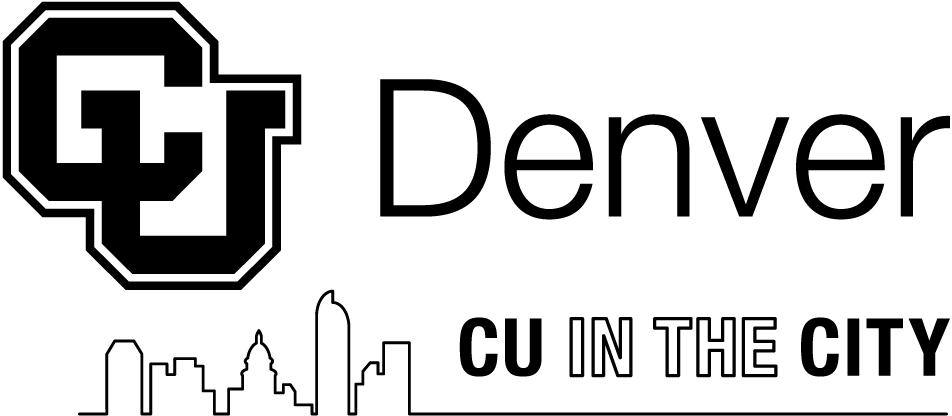
\includegraphics[width=1.25cm]{CUDenver-Logo.png}}
\rfoot{\mypage}
\cfoot{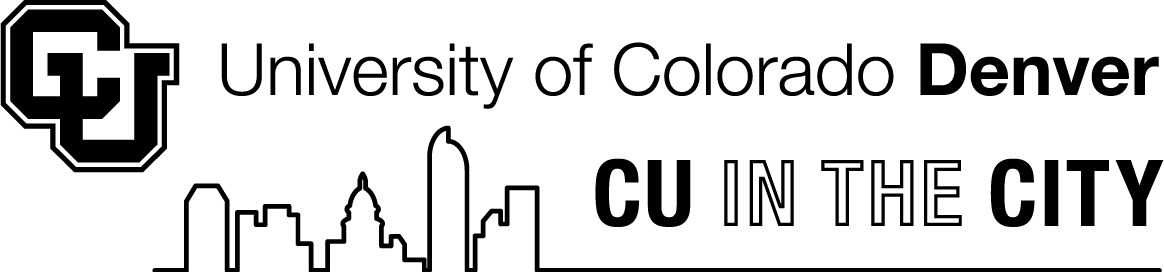
\includegraphics[width=2.25cm]{CUDenver-Logo-coverpage.png}}
\lfoot{Adam Spiegler}
\fancypagestyle{firstfooter}{\footskip = 50pt}
\renewcommand{\footrulewidth}{.4pt}
%%%%%%%%%%%%%%%%%%%%%%%%%%%
\vspace*{-20pt} \thispagestyle{firstfooter}


%\begin{tasks}[counter-format = {(tsk[a])},label-offset = {0.8em},label-format = {\color{black}\bfseries}](2)

\pagebegin{Section 6.1: Maximum Likelihood Estimation (MLE)}

\bb
\ii A strategic gambler believes they have identified a faulty slot machine which pays out significantly  more money than the other slot machines. She and her friends watch the machine 24 hours a day for 7 days and observed the slot machine paid out the \$$1,\!000,\!000$ jackpot prize 10 times during the week. How can she figure out whether the machine is faulty or whether the number of jackpot prizes are within reason?

\bb
\ii \colorr{Collect data:} They decide to compare the performance of the suspect slot machine to other slot machines. They pick a random sample of 4 other slot machines and record how many jackpot prizes each machine pays over a one week time frame: %Let random variable $X$ denote the number of jackpots paid out per week by a randomly selected slot machine.
\[ x_1=1 \ ,\  x_2=3\ ,\  x_3=4 \ , \ x_4=8 \]

\ii \colorr{What model best fits the data?}%If we had a larger dataset, we could visualize the data. Based on this context what discrete random variable model would make sense?

\bs
\colorr{Poisson Distribution}

\bs

\ii \colorr{Determine the value of the parameter(s) of the model:} Given the observed data, what are the most likely values of the parameters?

\vspace{1.15in}

\ee
\ee

\bbox
The \colorb{\textbf{likelihood function}} $L(\theta)= L( \theta \mid x_1, x_2, \ldots x_n)$ gives the likelihood of the
parameter $\theta$ given the observed data. A \colorb{\textbf{maximum likelihood estimate, $\mathbf{\hat{\theta}_{\rm MLE}}$,}} is
a value of $\theta$ that maximizes the likelihood function.

\textbf{MLE is a process for finding the best parameter(s) for a model based on a given dataset. } 
\ebox

\bb[resume]
\ii Find the value of $\lambda$ that maximizes the likelihood function from question 1.
\ee

\hspace{4in} 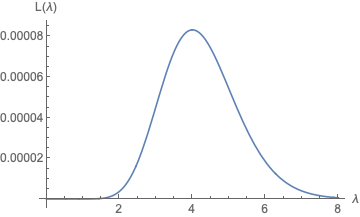
\includegraphics[width=2.5in]{14/fig-slot-mle.png}

\vfill


\clearpage


\pagebegin{Deriving the Likelihood Function}

 \bbox
Let $f(x; \theta)$ denote the pdf of a random variable $X$ with associated parameter $\theta$. Suppose
$X_1, X_2, \ldots , X_n$ are random samples from this distribution, and $x_1, x_2, \ldots , x_n$ are the
corresponding observed values.

\[ L(\theta \mid x_1, x_2, \ldots , x_n) = f(x_1; \theta) f(x_2; \theta) \ldots f(x_n; \theta) = \prod_{i=1}^n f(x_i; \theta).\]
\ebox

\bb[resume]
\ii For the following random samples, find the likelihood function:
\bb
\ii $(x_1, x_2, x_3, x_4) = (1,3,3,2)$ comes from $X \sim \mbox{Binom}(3,p)$. \vfill
\ii $x_1, x_2, x_3, \ldots, x_n$ come from $X \sim \mbox{Exp}(\lambda)$.  \vfill
\ee


\clearpage

\pagebegin{Maximizing the Likelihood Function}

\ii Find the MLE for $p$ when  $(x_1, x_2, x_3, x_4) = (1,3,3,2)$ comes from $X \sim \mbox{Binom}(3,p)$.

\ee

\vfill

\hspace{3in} 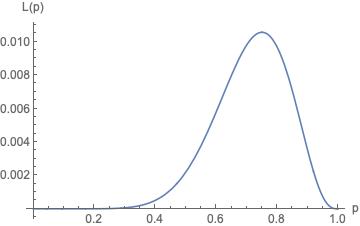
\includegraphics[width=2.5in]{14/fig-binom-mle.png}

\bs

 \bbox
Steps for finding MLE, $\hat{\theta}_{\rm MLE}$:
\bb
\ii Find a formula the likelihood function.
\[ L(\theta \mid x_1, x_2, \ldots , x_n) = f(x_1; \theta) f(x_2; \theta) \ldots f(x_n; \theta) = \prod_{i=1}^n f(x_i; \theta) \]
\ii Maximize the likelihood function.
\bb
\ii Take the derivative of $L$ with respect to $\theta$
\ii Find critical points of $L$ where $\frac{dL}{d\theta}=0$ (or is undefined).
\ii Evaluate $L$ at each critical point and identify the MLE.
\ee
\ee
\ebox

\clearpage

\bb[resume]
\ii Find the MLE for $\lambda$ when $x_1, x_2, x_3, \ldots, x_n$ comes from $X \sim \mbox{Exp}(\lambda)$.

 \vfill

\ee

\bbox
The value of $\theta$ that maximizes the \colorb{\textbf{log-likelihood function}} $y = \ln{\bigg( L(\theta \mid x_1, x_2, \ldots , x_n) \bigg)}$ will also the value that maximizes $L(\theta \mid x_1, x_2, \ldots , x_n)$.
\ebox

\clearpage

\pagebegin{Practice}

\bb[resume]
\ii Suppose a random variable with $X_1=5$, $X_2=9$, $X_3=9$, and $X_4=10$ is drawn from a distribution with pdf
\[ f( x; \theta) = \frac{\theta}{2\sqrt{x}}e^{-\theta \sqrt{x}}, \ \ \ \ \ \mbox{where x $>0$}.\]
Find an MLE  for $\theta$.
\ee


\vfill

\hspace{3in} 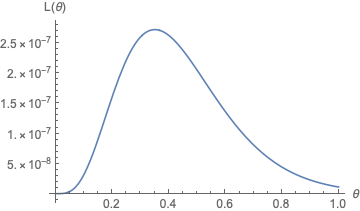
\includegraphics[width=2.5in]{14/fig-theta-mle.png}

\clearpage

\pagebegin{Summary of Results}

 So far we have observed:
  \begin{center}
    \begin{tabular}{l|c}
      Distribution & $\dsty \hat{\theta}_{\rm MLE}$ \\
      \hline
      Binomial & $\dsty \hat{p}_{\rm MLE} = \hat{p}$ \\
      \hline
      Exponential & $\dsty \hat{\lambda}_{\rm MLE} = \frac{1}{\bar{x}}$
    \end{tabular}
  \end{center} 

  \bigskip

\bbox
  \begin{theorem}
    Let $x_1, x_2, x_3, \ldots, x_n$ be a random sample from $N(\mu, \sigma)$. The maximum likelihood estimates of $\mu$ and $\theta$ are
    \[ \hat{\mu} = \frac{1}{n} \sum_{i=1}^n x_i = \bar{x} \ \ \ \mbox{ and } \ \ \ \hat{\sigma} = \sqrt{\frac{1}{n} \sum_{i=1}^n (x_i - \bar{x})^2}.\]
  \end{theorem}
  \ebox

\bigskip


\bbox
\bi
\ii \colorb{\textbf{MLE's give reasonable estimates that make sense!}}
\ii MLE's are often good estimators since they satisfy several nice properties
\bi
\ii \textit{Consistency:}  As we get more data (sample size goes to infinity), the estimator becomes more and
more accurate and converges to the actual value of $\theta$.
\ii \textit{Normality:} As we get more data, the MLE's converge to a normal distribution.
\ii \textit{Efficiency:} They have the smallest possible variance for a consistent estimator.
\ei
\ii \colorr{\textbf{The downside is finding MLE's are not always easy (or possible).}}
\ei
\ebox


 
